%
%
\setcounter{section}{1}
\setcounter{prp}{3}
%
%----------------------------------------------
%
\section{\'Etude d'une fonction affine}
%\setcounter{subsection}{1}
%
%----------------------------------------------
%
%
%
\subsection{Variations}
%
%
\begin{prp}{}{} Soit une fonction affine $f\colon x\mapsto mx+p$.
\begin{itemize}
\item Si $m<0$ alors $f$ est (strictement) décroissante: \hfill
\begin{tikzpicture}[y=0.9cm,align at top]
\tikzset{arrow style/.style={black,%
					line width=0.75pt,->,%
					>= latex',%
					shorten >= 6pt,%
					shorten <= 6pt}}
\tkzTabInit[lgt=1.5,espcl=3]%,deltacl=0.4
{$x$/0.5,$f(x)$/1.25}{$-\infty$,$+\infty$}%
\tkzTabVar{+/ ,-/ }%
\end{tikzpicture}
\item Si $m>0$ alors $f$ est (strictement)  croissante: \hfill
\begin{tikzpicture}[y=0.9cm,align at top]
\tikzset{arrow style/.style={black,%
					line width=0.75pt,->,%
					>= latex',%
					shorten >= 6pt,%
					shorten <= 6pt}}
\tkzTabInit[lgt=1.5,espcl=3]%,deltacl=0.4
{$x$/0.5,$f(x)$/1.25}{$-\infty$,$+\infty$}%
\tkzTabVar{-/ ,+/ }%
\end{tikzpicture}
\item Si $m=0$ alors $f$ est  constante: \hfill
\begin{tikzpicture}[y=0.9cm,align at top]
\tikzset{arrow style/.style={black,%
					line width=0.75pt,->,%
					>= latex',%
					shorten >= 6pt,%
					shorten <= 6pt}}
\tkzTabInit[lgt=1.5,espcl=3]%,deltacl=0.4
{$x$/0.5,$f(x)$/1}{$-\infty$,$+\infty$}%
\tkzTabVar{+/ ,+/ }%
\end{tikzpicture}
\end{itemize}
\end{prp}
%
%
%
%
%
%
\subsection{Signes}
\setcounter{prp}{6}
%
%
\begin{prp}{}{} Soit une fonction affine $f\colon x\mapsto mx+p$.
\begin{itemize}
\item Si $m<0$ alors : \hspace*{0.5cm}
\begin{minipage}[c]{0.7\linewidth}
{\centering
\begin{tikzpicture}
\tkzTabInit[lgt=3,espcl=3]{$x$ /0.75%
				, signe de $f(x)$ /0.75}%
{$-\infty$,$-\frac{p}{m}$,$+\infty$}%
\tkzTabLine{ , + , z ,- , }
\end{tikzpicture}

} 
\end{minipage}
  \item Si $m>0$ alors : \hspace*{0.5cm}
\begin{minipage}[c]{0.7\linewidth}
{\centering
\begin{tikzpicture}
\tkzTabInit[lgt=3,espcl=3]{$x$ /0.75%
				, signe de $f(x)$ /0.75}%
{$-\infty$,$-\frac{p}{m}$,$+\infty$}%
\tkzTabLine{ , - , z , + , }%\noexpand\pointille{$-\frac{p}{m}$}
\end{tikzpicture}

}
\end{minipage}
\end{itemize}
\end{prp}